Partie-Vorbereitung

FA-G \ref{Partie-Vorbereitung} %FA-G 126 Partie-Vorbereitung

Wahlphase

FA-G \ref{Charakter} %FA-G 64 Charakter 
FA-G \ref{Charakter Liste} %FA-G 65 Charakter Liste
FA-G \ref{Gadgets} %FA-G 94 Gadgets
FA-G \ref{Wahlphase} %FA-G 127 Wahlphase

Ausrüstungsphase
FA-G \ref{Inventar} %FA-G 74 Inventar
FA-G \ref{Gadgets} %FA-G 94 Gadgets
FA-G \ref{Ausruestungsphase} %FA-G 128 Ausrüstungsphase

Startplatzverteilung der Charaktere

FA-S \ref{s-partieinit} %FA-S 8 Spiel Start und Initialisierung
FA-G \ref{Felder} %FA-G 53 Felder
FA-G \ref{Spielbrett} %FA-G 54 Spielbrett

Zugreihenfolge festlegen

FA-S \ref{s-rundeinit} %FA-S 9 Rundenstart und Initialisierung

Spiel pausieren

FA-S \ref{s-rundeinit} %FA-S 12 Spielpause
FA-C \ref{c-pause} %FA-C 32 Wunsch auf Pausieren
FA-C \ref{c-unpause} %FA-C 33 Wunsch auf Wiederaufnahme des Spiels

Spiel fortsetzen

FA-S \ref{s-rundeinit} %FA-S 12 Spielpause
FA-C \ref{c-unpause} %FA-C 33 Wunsch auf Wiederaufnahme des Spiels

Spielbrett aktualisieren

FA-S \ref{s-state-senden} %FA-S 14 Senden des Spielzustands
FA-C \ref{c-gui} %FA-C 27 Spiel Anzeige
FA-G \ref{Spielbrett} %FA-G 54 Spielbrett

Spielbrett anzeigen

FA-C \ref{c-gui} %FA-C 27 Spiel Anzeige
FA-G \ref{Spielbrett} %FA-G 54 Spielbrett

Charakter anzeigen 

FA-C \ref{c-gui} %FA-C 27 Spiel Anzeige
FA-G \ref{Charakter} %FA-G 64 Charakter 

Feld anzeigen

FA-C \ref{c-gui} %FA-C 27 Spiel Anzeige
FA-G \ref{Felder} %FA-G 53 Felder

Spielzustand aktualisieren

FA-S \ref{s-state-senden} %FA-S 14 Senden des Spielzustands

Spielzug durchführen

FA-S \ref{s-spiel} %FA-S 10 Spiel Durchführung

Spielzug animieren

FA-C \ref{c-animation} %FA-C 31 Animation der Aktionen

Spielzug validieren

FA-S \ref{s-regeln} %FA-S 13 Erkennung von Regelverstößen

Punkt verwenden

FA-G \ref{BP und AP} %FA-G 69 Bewegungspunkte (BP) und Aktionspunkte (AP)

Bewegung durchführen

FA-G \ref{Bewegung durchfuehren} %FA-G 115 Bewegung durchführen

Drängeln

FA-G \ref{Draengeln} %FA-G 116 Drängeln

Gewinner Erkennung

FA-S \ref{s-gewinner} %FA-S 15 Gewinner Erkennung

Gewinner anzeigen

FA-C \ref{c-winnerdisplay} %FA-C 37 Gewinneranzeige

Charakter auswählen

FA-G \ref{Charakter-Position} %FA-G 67 Charakter-Position

Charakterwert anzeigen

FA-G \ref{Charakter} %FA-G 64 Charakter 

Aktion durchführen

FA-G \ref{Aktion durchfuehren} %FA-G 117 Aktion durchführen

freies Nachbarfeld finden

FA-S \ref{s-alternatives} %FA-S 11 Finden freier Felder und Alternativen

Gadget verwenden

FA-G \ref{Gadget verwenden} %FA-G 118 Gadget verwenden
FA-G \ref{Gadgets} %FA-G 94 Gadgets

Roulette spielen

FA-G \ref{Roulette spielen} %FA-G 119 Roulette spielen

Charaktereigenschaft anwenden

FA-G \ref{Eigenschaften} %FA-G 73 Eigenschaften
FA-G \ref{Bang and Burn} %FA-G 90 Bang and Burn
FA-G \ref{Observation} %FA-G 93 Observation

Spionieren

FA-G \ref{Spionieren} %FA-G 123 Spionieren

Tresor spicken

FA-G \ref{Tresor-Spicken} %FA-G 124 Tresor-Spicken

Tresorkombination erhalten

FA-G \ref{Geheimnis erhalten} %FA-G 125 Geheimnis erfahren

Cocktail-Aktion durchführen

Cocktail aufnehmen

FA-G \ref{Cocktail aufnehmen} %FA-G 120 Cocktail aufnehmen
FA-G \ref{haelt Cocktail} %FA-G 75 hält Cocktail

Jemanden mit einem Cocktail übergießen

FA-G \ref{haelt Cocktail} %FA-G 75 hält Cocktail
FA-G \ref{Cocktail-Guss} %FA-G 121 Cocktail-Guss

Cocktail schlürfen

FA-G \ref{haelt Cocktail} %FA-G 75 hält Cocktail
FA-G \ref{Cocktail schluerfen} %FA-G 122 Cocktail schlürfen



\begin{figure}
  \centering
  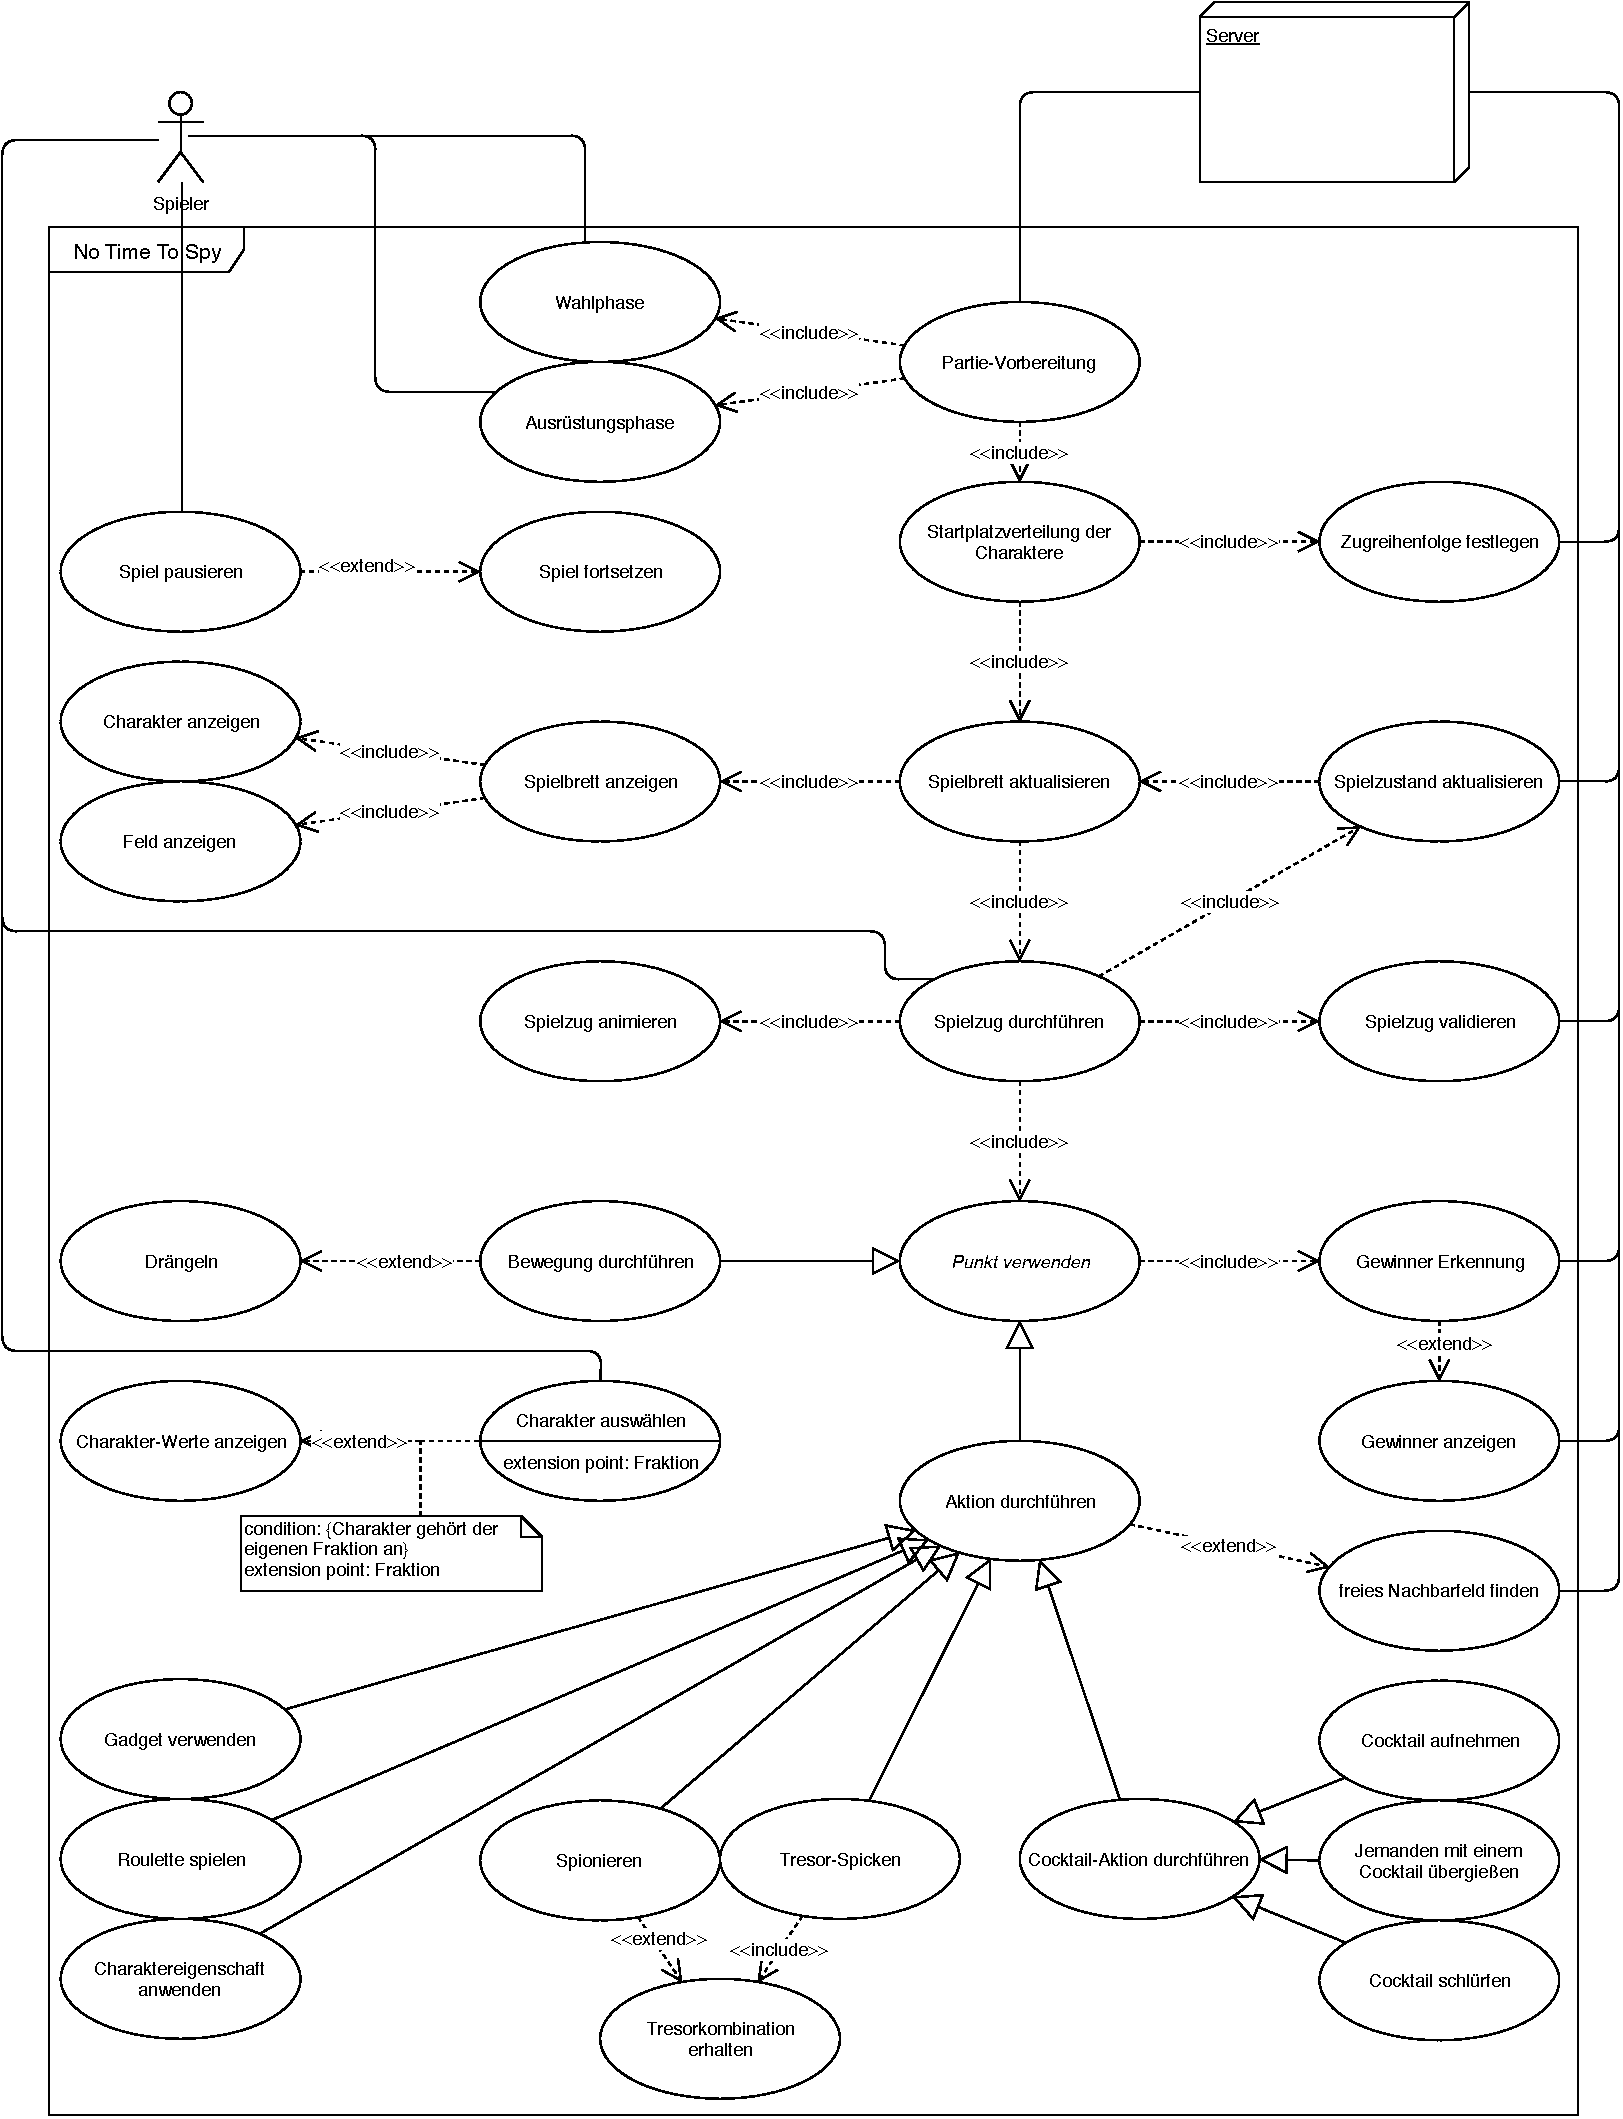
\includegraphics[width=\textwidth]{Meilenstein02/use_case_gamesession.pdf}
  \caption{Anwendungsfälle Spielpartie}
\end{figure}